%% !TEX root =  paper.tex

\section{Breakage Scenarios}\label{sec:study}

Given the predominance of locator-related issues, we focus our analysis on locator problems. We thus conducted a study to categorize the breakages from a repair-oriented perspective. 
While there exist taxonomies related to web and GUI breakages~\cite{Hammoudi-2016-ICST,Issa:2012:VTG:2412102.2412107,7102582}, none of them are detailed enough as far as automatic repair is concerned. 
The findings from this study highlight the complexity and the variety of the breakages that can occur in E2E web tests, and that our approach aims to solve.

\subsection{A repair-oriented test breakages taxonomy}\label{sec:taxonomy}

\head{Study Setting}\label{sec:study}
In the intention of supporting a realistic test regression scenario, we selected open source web applications for which (i)~multiple versions and (ii)~Selenium test cases were available from previous research on web testing~\cite{WCRE}. %Especially the latter requirement was challenging, because non-trivial web test suites are rarely made publicly available, and in fact we found no open-source test suite of reasonable size for our study. Fortunately, we could select four web applications that have been used extensively in the context of previous research on web testing~\cite{WCRE}, and for which we were able to obtain four working Selenium test suites.

\autoref{table:subjectSystems} (Web Applications) shows information about the selected applications, including their names, the initial release for which the test suites were developed, the numbers of releases available after the initial release, and the number of lines of code (counted using \texttt{cloc}~\cite{cloc} and averaged across the releases).
\autoref{table:subjectSystems} (Test Suites) provides data on the test suites, including the total numbers of test cases counted across all versions along with the average number of test cases per version, and the total numbers of statements in all of the test cases counted across all versions along with the average number of statements per test case.

\begin{table}[h]
\setlength{\tabcolsep}{2pt}
\renewcommand{\arraystretch}{0.9}
\centering
%\footnotesize
\caption{Subject systems and their test suites}
\begin{tabular}{lrrr@{\hskip 2em}r@{\hskip 1em}r}
\toprule

& \multicolumn{3}{c}{\sc Web Applications} 
& \multicolumn{2}{c}{\sc Test Suites} \\

\cmidrule(r){2-4} \cmidrule(r){5-6}

& {\textbf{Init.}} 
& {\textbf{Rel.}}
& {\textbf{LOCs (K)}} 
& {\textbf{Tot/Avg}} 
& {\textbf{LOCs (K)}}   \\

\midrule
AddressBook   & 4.0       & 47       & 8,757   & 1,344/28        & 61,826/43          \\
Claroline     & 1.10.7    & 11       & 338,129 & 492/41        & 20,287/43          \\
Collabtive    & 0.65      & 13       & 150,696 & 560/40        & 22,710/38          \\
PPMA          & 0.2       & 11       & 556,164 & 276/23        & 16,732/47          \\
\midrule
Total/Average &           & 82       & 263,436 & 2,672/33        & 121,555/43 \\

\bottomrule
\end{tabular}
\label{table:subjectSystems}
\end{table}

\head{Procedure}\label{sec:procedure}
First, we determined the types of test breakages that occur in our objects of analysis. For each considered web application, for each version $V_n$ and its accompanying test suite $T_n$, we executed $T_n$ on the subsequent version $V_{n+1}$, and collected information about each breakage and each failure (e.g., actual bugs). We repeated this process until all the versions were taken into account. 

\begin{figure}[t]
\centering
%\fbox{
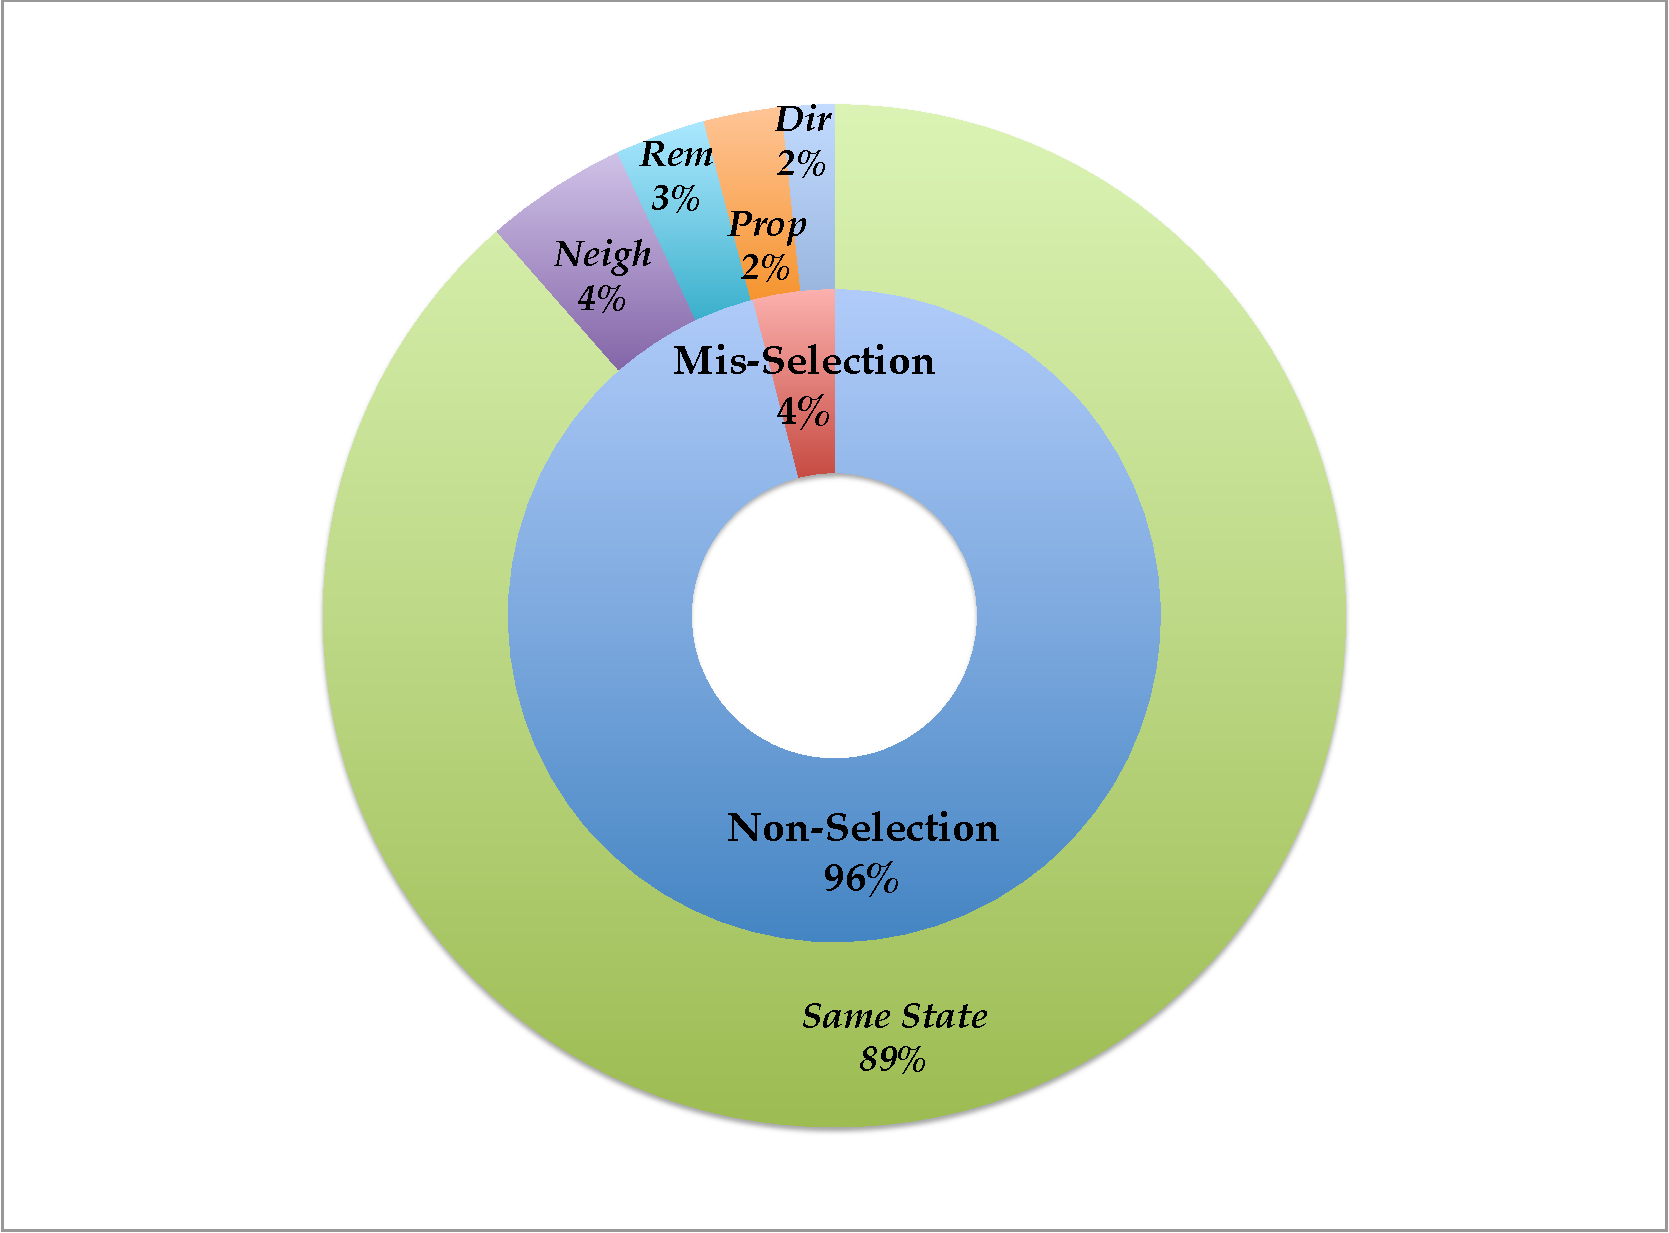
\includegraphics[trim={0cm 0cm 0cm 0cm},clip,scale=0.23]{images/donut}
%}
\caption{Distribution of Different Types of Breakages.}
\label{donut}
\end{figure}

\begin{figure}[b]
\centering
%\fbox{
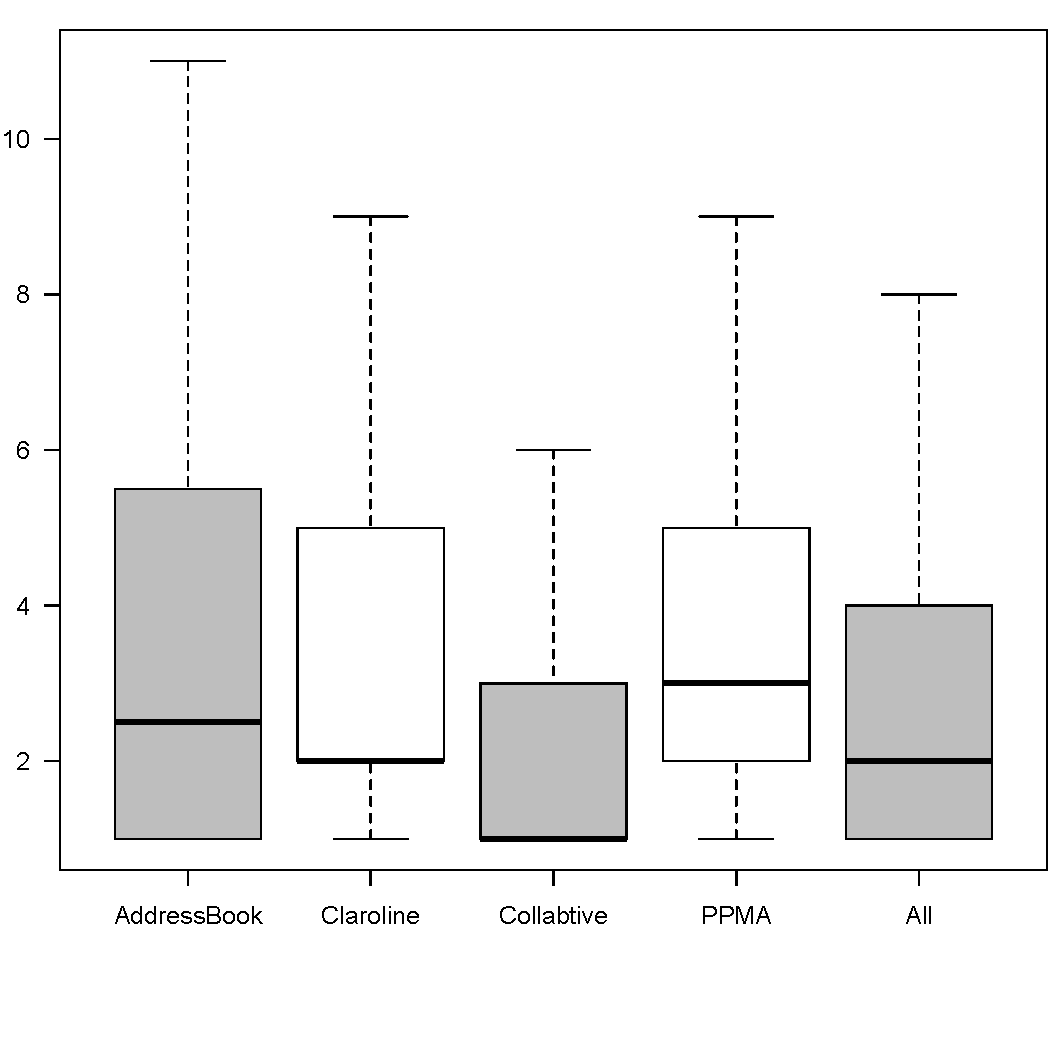
\includegraphics[trim={0cm 0cm 0cm 0cm}, clip,width=0.78\columnwidth]{images/distribution.pdf}
%}
\caption{Distribution of test breakages per test case in each subject system.}
\label{fig:distribution}
\end{figure} 

\begin{figure*}[h!]
\centering
\begin{subfigure}{\columnwidth}
\centering
%\fbox{
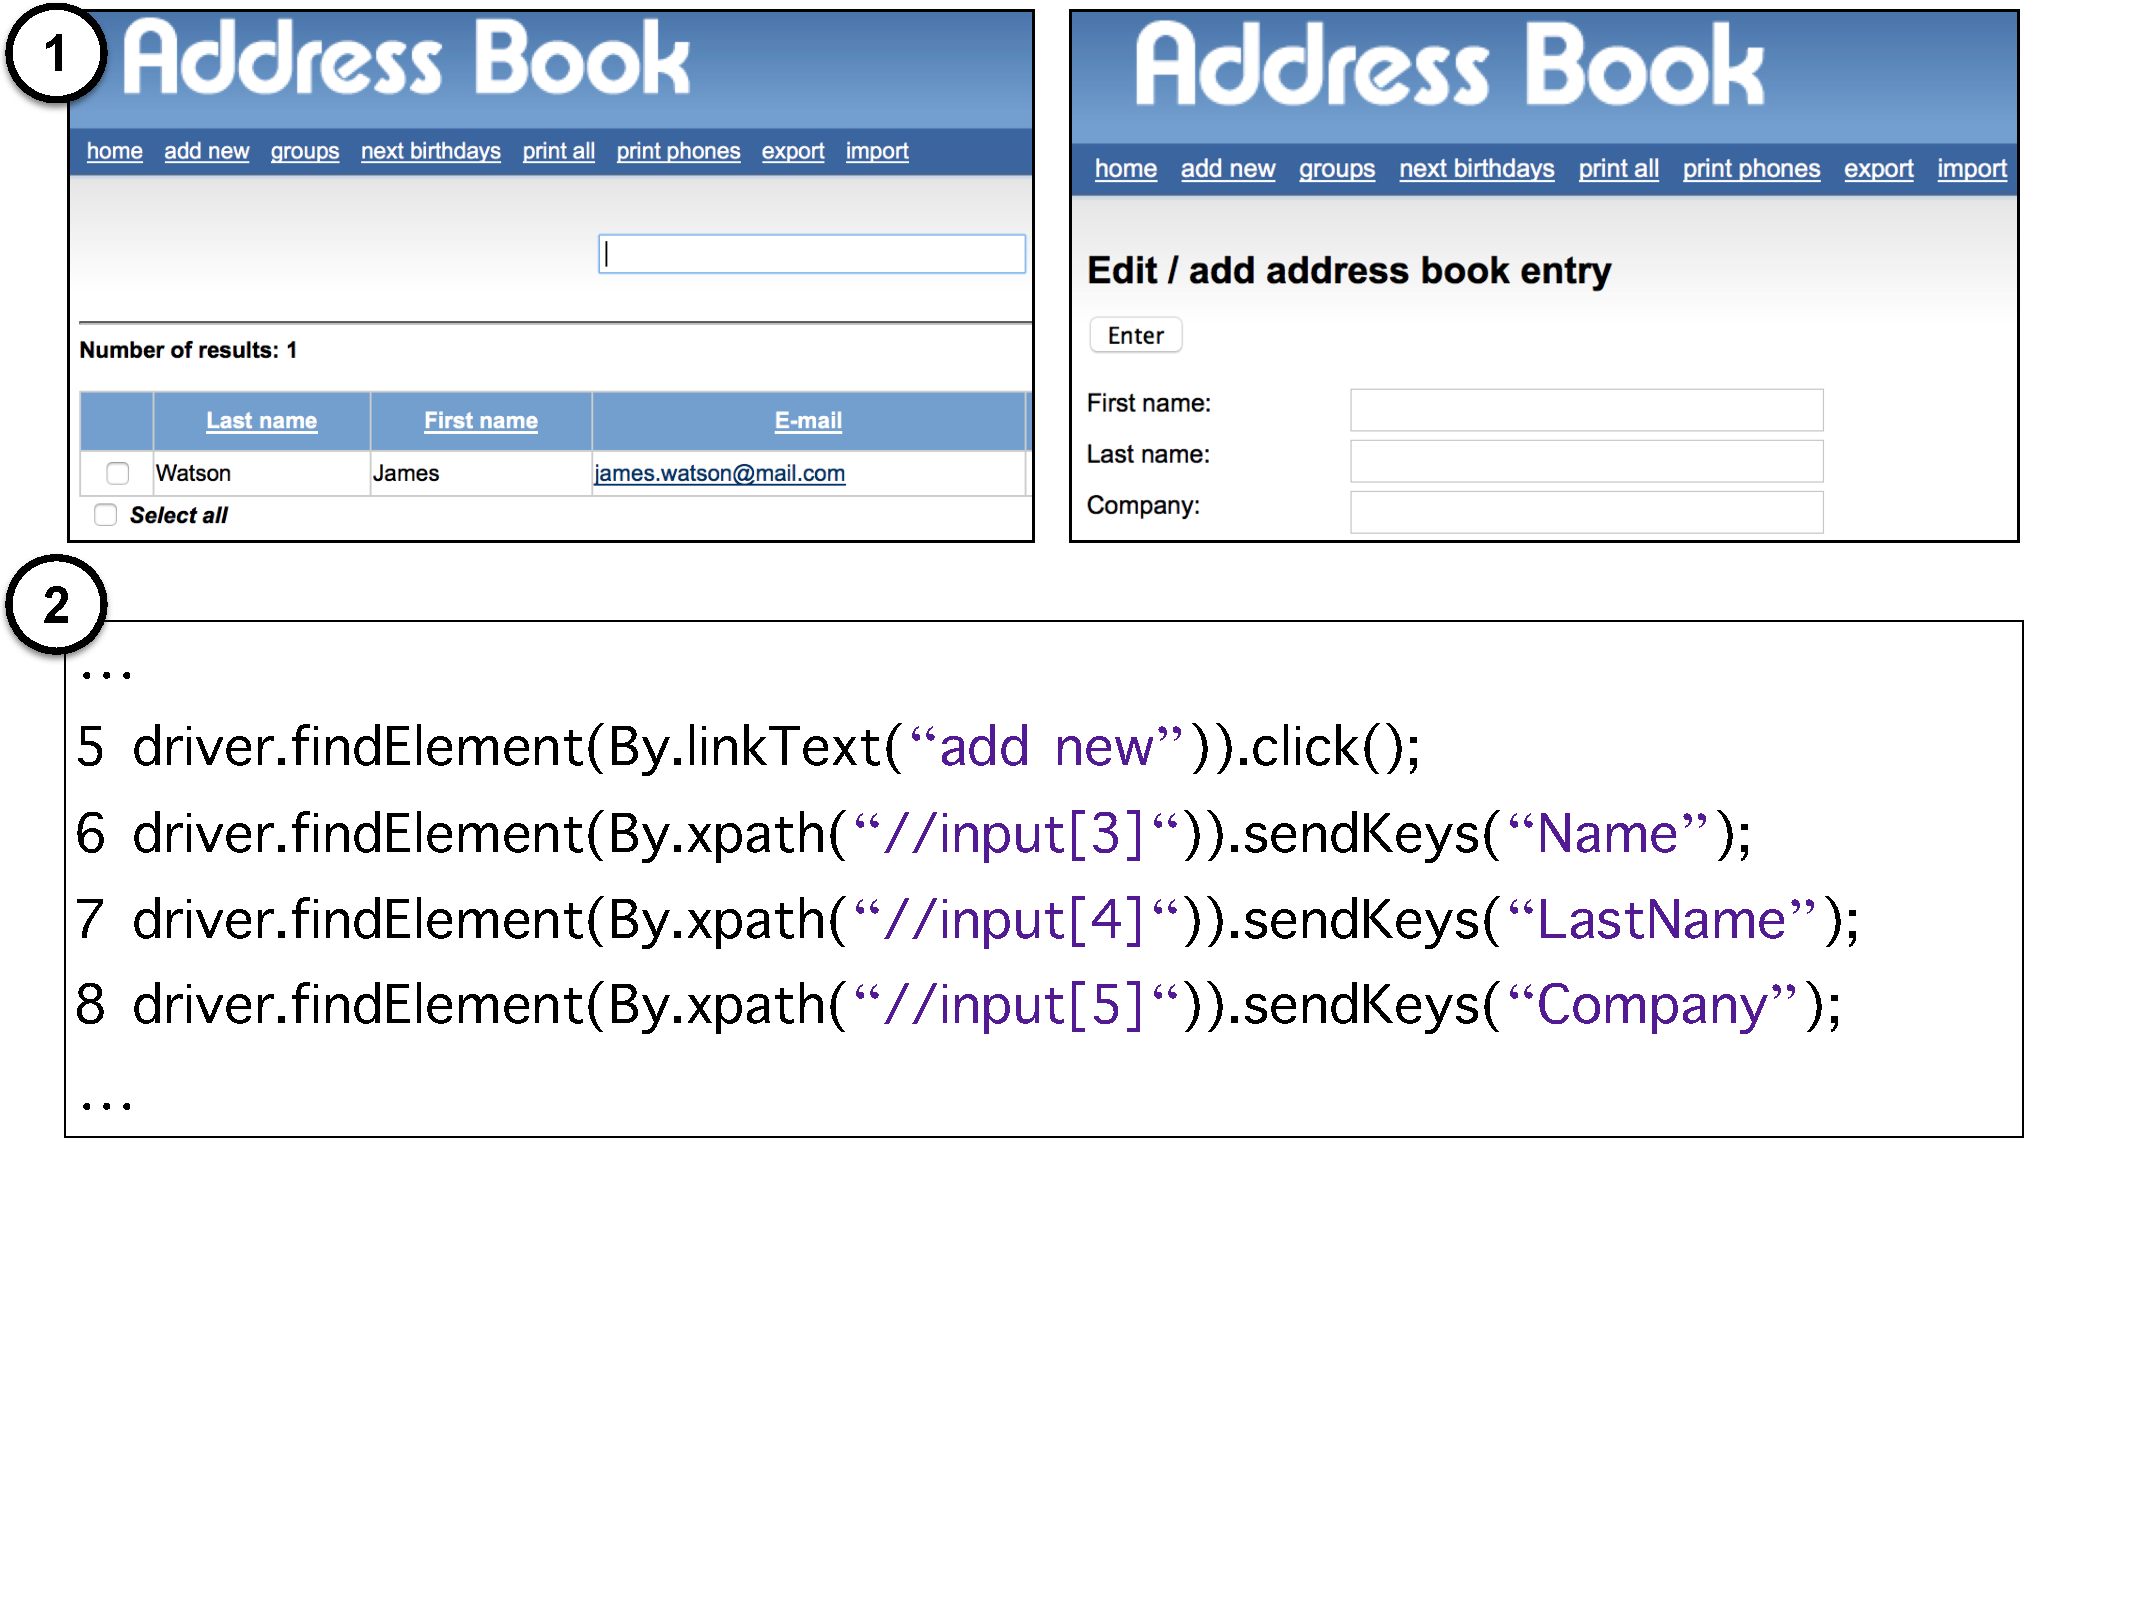
\includegraphics[trim=0cm 6cm 0cm 0cm, clip=true, scale=0.200]{images/addressbook-version1.pdf}
%}
\caption{\emph{Version 6.2.12}}
\label{fig:ab1} 
\end{subfigure}
\begin{subfigure}{\columnwidth}
\centering
%\fbox{
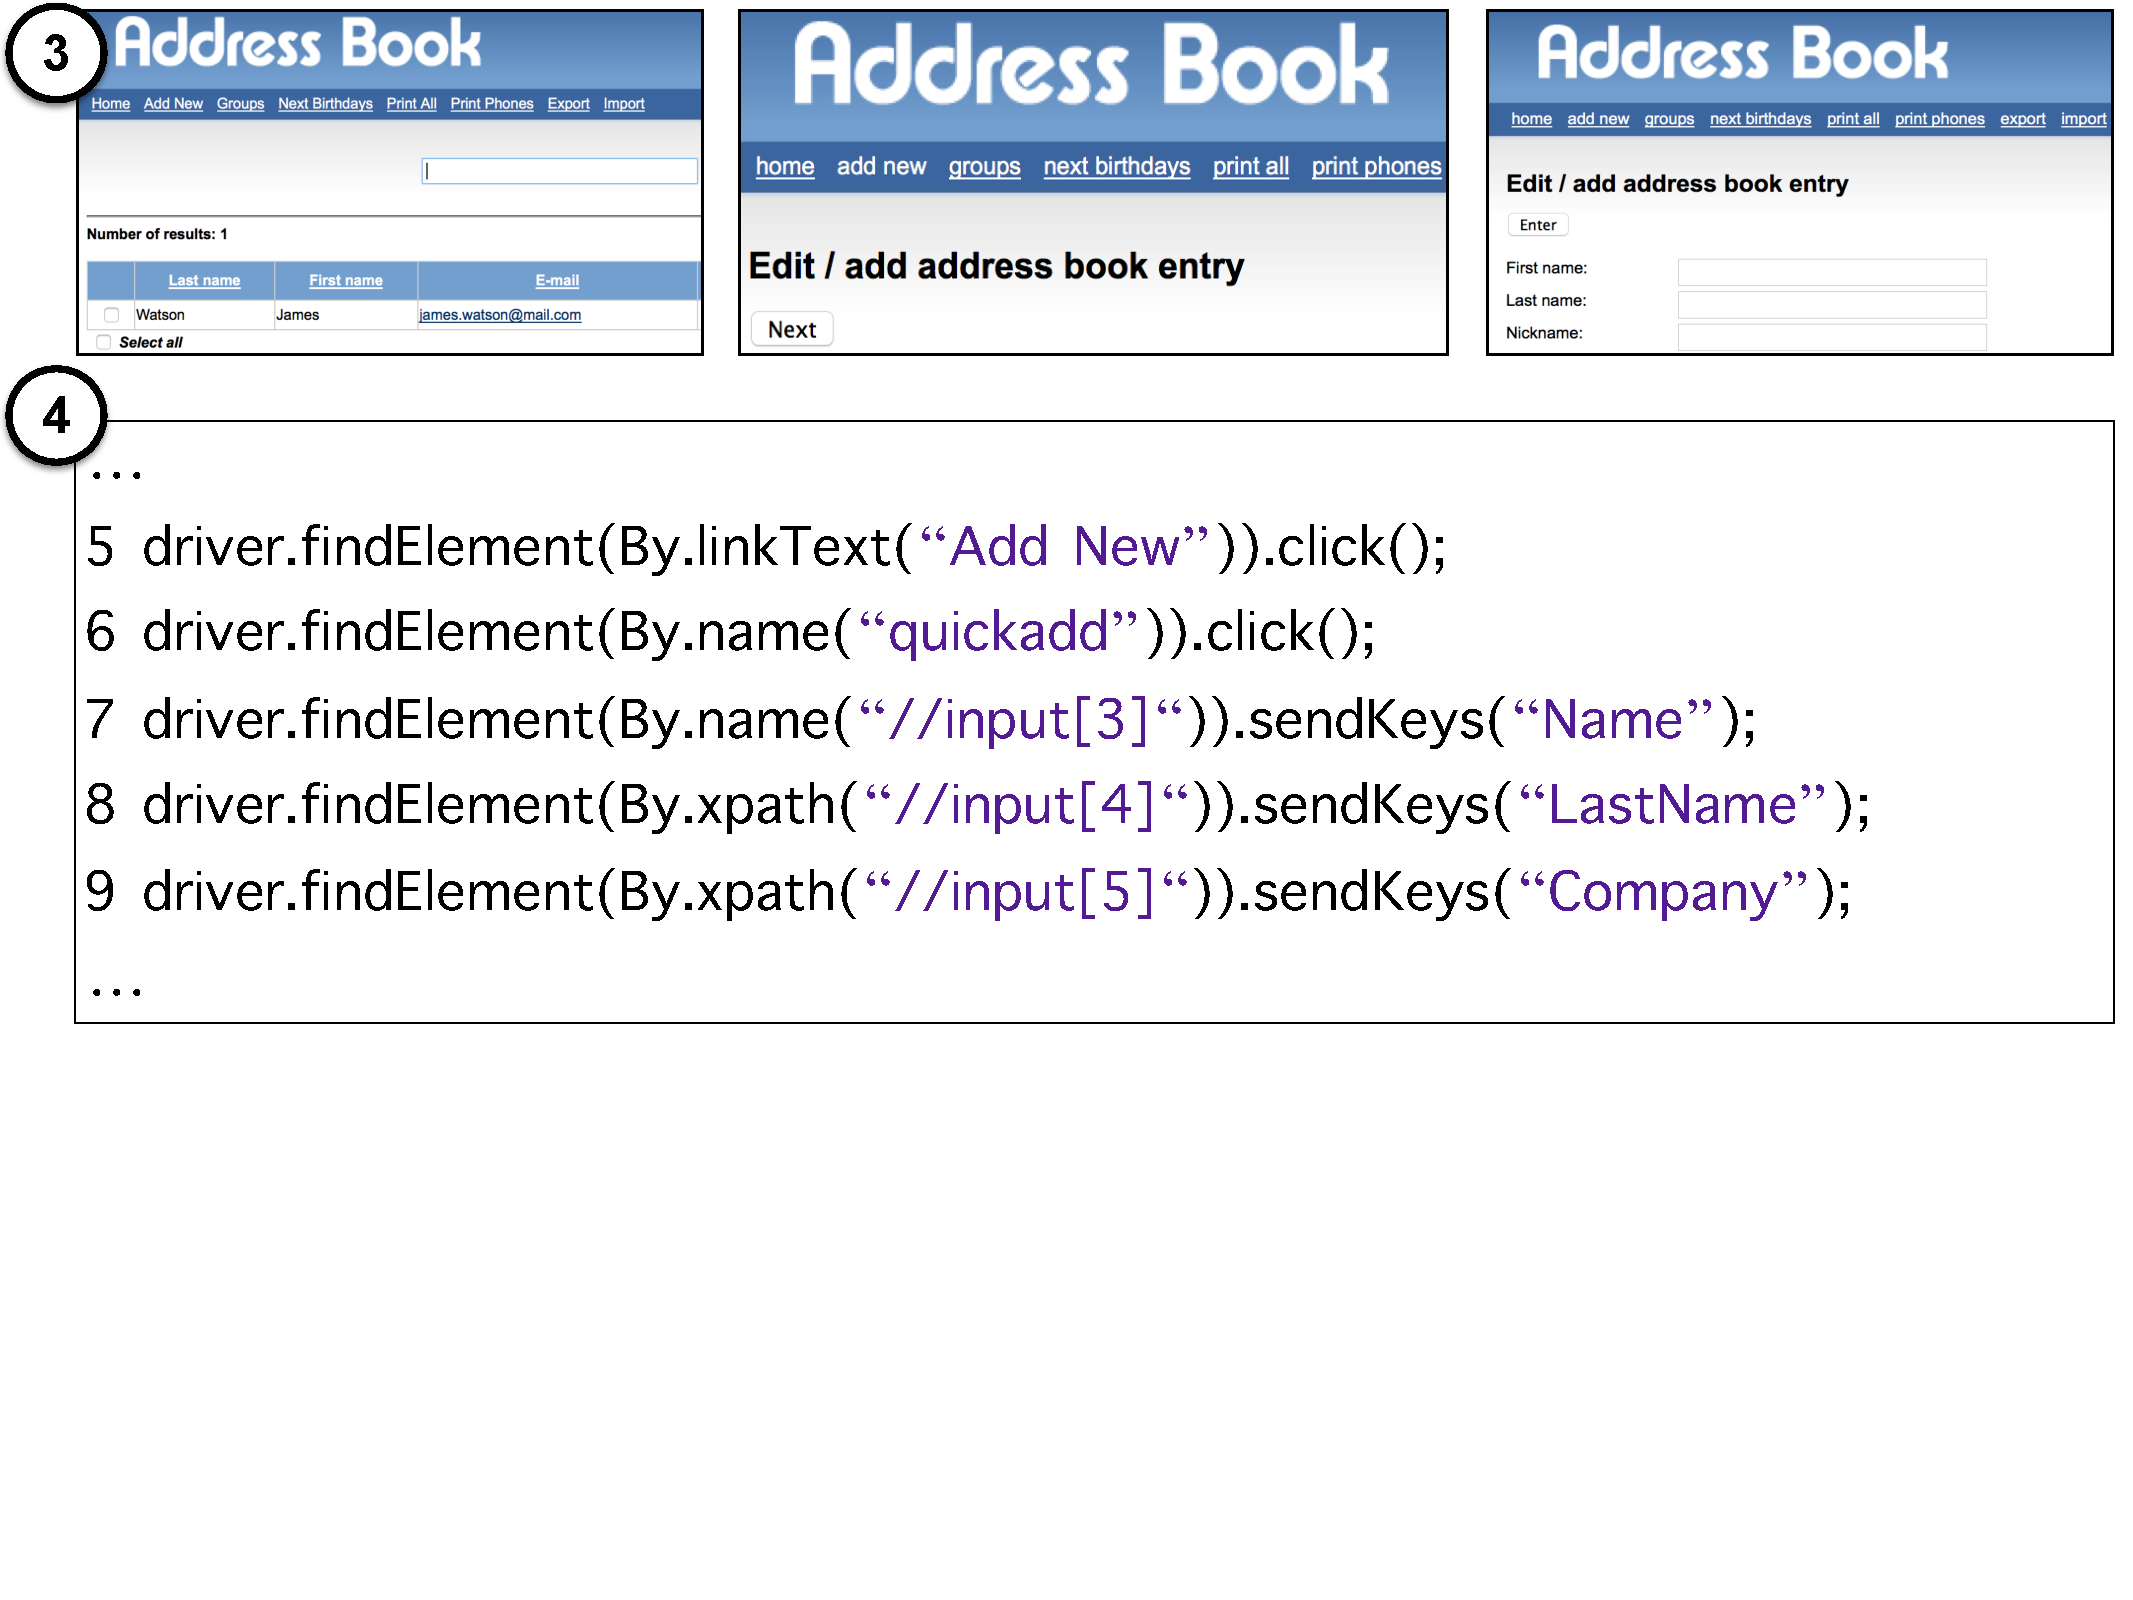
\includegraphics[trim=0cm 5cm 1.3cm 0cm, clip=true,  scale=0.190]{images/addressbook-version2.pdf}
%}
\caption{\emph{Version 7.0.0}}
\label{fig:ab2}
\end{subfigure}
\caption{AddressBook web application, version 6.2.12 (\ref{fig:ab1}) and version 7.0.0 (\ref{fig:ab2}), along with Selenium WebDriver tests.} 
\label{fig:example} 
\end{figure*}

\head{Grounded Theory Study Results}\label{sec:study}
We collected 733 individual test breakages, distributed as follows: 50 for AddressBook, 165 for Claroline, 218 for Collabtive, and 300 for PPMA.
\autoref{donut} shows the distribution of the different types of locator breakages. Our study revealed two major categories, each of which has specific subtypes. The most prevalent category refers to \textit{Non-Selection} of web elements (695/733). Among those, $\approx$93\% are related to web elements that are still on the same web page (or test state), $\approx$5\% pertain to web elements that are moved to a neighbouring web page (or test state), and $\approx$2\% to web elements being removed from any web page.
The second main category consists of \textit{Mis-Selection} of web elements (38/733), of which $\approx$68\% led to \textit{direct} breakages, and $\approx$32\% to \textit{propagated} breakages. 
Additionally, we collected 94 test \textit{failures}---meaning the tests exposing actual bugs---and 22 failures due to obsolete \textit{assertion} values.
%
That said, in the context of this paper, we focus on repairing the regression breakages. 

\autoref{fig:distribution} shows box-plots about the distribution of breakages per test cases in each subject system. We observe that on average between 1--4 breakages are present per test. 
In short, (1)~test suites tend to break frequently as the web application evolves, and (2)~breakages may pertain occur multiple times within the same test. 
In the following of this section, we detail the test breakage scenarios by means of a running example.

\subsection{Breakage Scenarios}\label{sec:breakage-scenarios}

\noindent
\textbf{Basic Terminology.}
At a high level, each web test statement is a tuple \textit{<locator, action, value>}. 
The locator component specifies the web element the test statement is interacting with. A locator $l$ is a function on a DOM state $\mathcal{D}$. Notationally, $l: \mathcal{D} \rightarrow \{e\}$ where $e$ is the web element returned by the locator $l$ when applied to $\mathcal{D}$. 
%
%Locator breakages are due to one or more DOM-based root causes. A root cause is a tuple $<\mathcal{D}, e, a, v>$ where $\mathcal{D}$ is a DOM tree (e.g., a test state), $e$ is the web element in $\mathcal{D}$ on which the test currently operates, $a$ is a HTML attribute of $e$, and $v$ is the value of $a$. 
%We define a repair as a tuple $<r, e', a', v', \mathcal{D'}>$, where $r$ is a root cause and $e'$ is the suggested new web element for $\mathcal{D}$ in the root cause $r$, having attribute $a'$ set to $v'$. 
%The locator function is surjective, that is every web element $e$ is mapped to by at least one locator (e.g., the XPath from the root to $e$), but there exist multiple locators {$\displaystyle \forall l\in L,\exists e\in D{\text{ such that }} l: D \rightarrow \{e\}$}.



\noindent
\textbf{Scenario 1 (Non-Selection $\bullet$ Same State).}
A non-selection occurs when a locator $l$ applied to a DOM state $\mathcal{D}$ returns no elements---formally, $l: \mathcal{D} \rightarrow \emptyset$, but the target element $e$ is still present on the page ($e \in \mathcal{D}$).
Then, possible repairs require to find another locator $l' \mid l': \mathcal{D} \rightarrow e$.

As an example, consider the login page of AddressBook in~\autoref{fig:ab1}~\textcircled{\raisebox{-0.8pt}{1}}, and the accompanying WebDriver test~\textcircled{\raisebox{-0.8pt}{2}}. 
%, which was developed for (or evolved until) version 6.2.12, where it runs correctly.
%\textcircled{\raisebox{-0.8pt}{1}}~shows the home page of AddressBook web application version 6.2.12, and the page in which the user can insert a new entry. A portion of a possible Selenium WebDriver test script is also shown~\textcircled{\raisebox{-0.8pt}{2}}, which was developed for (or evolved until) version 6.2.12, where it runs correctly.
%
Suppose that in the new subsequent version of AddressBook (7.0.0), as a result of the application evolution, 
the login button gets modified as follows: \code{<input value=``Login''></input>} becomes \code{<button>Login</button>}.
%\texttt{id=``submitLogin''}. In particular, the menu bar items have been capitalized, and a new confirmation page has been added before the insert entry page. 
%Finally,~\textcircled{\raisebox{-0.9pt}{4}} shows a portion of a Selenium WebDriver test~\cite{selenium} which fills in the username and password input boxes (Lines~5-6), and submits the form (Line~7). Suppose the test was developed for (or evolved until) version 1.10.0, where it ran correctly.

When executed on version 7.0.0, the test~\textcircled{\raisebox{-0.8pt}{2}} will then stop at Line~4 when attempting to locate the login button. %Non-selection problems manifest as \textit{direct} breakages, because the broken statement is the one that needs to be repaired.  
%
At a visual inspection of the two GUIs, a tester would expect the test to work, because her perception is immaterial where changes at DOM-level are concerned. It is indeed evident that the target element is \textit{visually} still present on the page, and its position \textit{on the GUI} has not changed.
 

%At this aim, a tester may wish to use the \water  technique~\cite{Choudhary:2011:WWA:2002931.2002935} to automatically repair the broken statement. Specifically, another locator for the ``Login'' button needs to be found, rather the relying on ``broken'' \texttt{value} attribute. \water will attempt to gather information about the broken element (such as the XPath, and the various attributes) by analysing the DOM of the previous version, and match such information on the evolved DOM of version 7.0.0. Unfortunately, \water's technique is ineffective in such a scenario, because (1)~the attribute \texttt{value} has been deleted from the DOM, and (2)~the XPath and the tag of the target element have changed (from \mbox{\texttt{input}} to \mbox{\texttt{button}}), which renders impossible for \water's heuristic to identify it on the evolved DOM. 
 
%\noindent
%\textit{Visual-aided Mitigation.}
%In this case, an algorithm taking into consideration the visual appearance of the test state might be able to match the target element between the two GUIs (in a similar way as a human would do). However, this task is challenging to be automated because several issues needs first to be solved. Among all (1)~finding an accurate visual matching technique, and, in the case a visual match is found, (2)~retrieving the corresponding element in the DOM. 

\noindent
\textbf{Scenario 2 (Non-Selection $\bullet$ Neighbouring State).}
Notationally this can be expressed as $l: \mathcal{D} \rightarrow \emptyset \land \exists \ \mathcal{D'} \mid l: \mathcal{D'} \rightarrow \{e\}$.
As a concrete example consider \autoref{fig:ab1}~\textcircled{\raisebox{-0.7pt}{1}}, %showing Addressbook web application version 6.2.12, 
specifically the pages in which the user can insert a new entry. The test~\textcircled{\raisebox{-0.7pt}{2}} clicks on the ``add new'' link on the home page (Line~5), and fills in the ``First name'', ``Last name'' and ``Company'' text fields (Lines~6--8).
Suppose now to replay this test on the successive version 7.0.0~\textcircled{\raisebox{-0.7pt}{3}}, for regression purposes. The test will raise an exception of kind \texttt{NoSuchElementException} at Line~6, when attempting to locate the ``First name'' text field~\textcircled{\raisebox{-0.7pt}{2}}. 
Indeed, a new intermediate confirmation page has been added~\textcircled{\raisebox{-0.9pt}{3}}, and the navigational workflow of the test must be corrected to reflect that of the new  web application.

From a testing perspective, the ``First name'' text field can no longer be found on the web page (test state) following the execution of the statement at Line~5. However, conceptually, the repair action that needs to be triggered in order to correct the test has nothing to do with the locator at Line~6.
In fact, by only looking at the exception, it is arduous for the tester to understand what the actual problem is, unless the \textit{visual execution} of the test is taken into consideration.
%
%Even the use of \water is unsuccessful, because it would attempt at repairing the broken statement at Line~6. (the technique only handles addition of statements within forms, and does not apply to general broken workflow scenarios).
%
%\noindent
%\textit{Visual-aided Mitigation.}
A possible solution would require to (1)~detect that the web element $e$ no longer exists as part of the test state $st_i$ in version $V$, (2)~try to match the $e$ in one of the neighbouring states of $st_i$ in the new version $V'$, which requires to (3)~find  a web element $e' \in st_i$ such that $(e', st_i) \rightarrow st_j$ (the ``Next'' button in our example~\textcircled{\raisebox{-0.7pt}{3}}).

\noindent
\textbf{Scenario 3 (Non-Selection $\bullet$ Removed).} 
%
The third and last \textit{Non-Selection} scenario concerns a web element being removed from a web page. Formally, $l: \mathcal{D} \rightarrow \emptyset \land \nexists \ \mathcal{D'} \mid l: \mathcal{D'} \rightarrow \{e\}$.
In a way, this can be seen as the opposite scenario of Scenario 2. 
As a concrete example, consider the example of \autoref{fig:ab2}, with the application being evolved in the reverse order as depicted in the figure (thus considering going from version 7.0.0 to version 6.2.12). The test~\textcircled{\raisebox{-0.7pt}{4}} would stop at Line 6, when trying to select the ``Next'' button, which was on a page that is no longer present. In this case, the only possible fix is to delete the statement.

%\noindent
%\textit{Visual-aided Mitigation.}
%A possible solution would require to (1)~search for the the web element $e$ both in $st_i$ and its neighbouring states, and (2)~if not match is found, then remove the statement.

\noindent
\textbf{Scenarios 4 and 5 (Mis-Selection $\bullet$ Direct and Propagated).}\label{sec:misselection}
In web testing, it is frequent for web elements to get repositioned in the DOM tree. This can cause locators to ``mis-select'' elements.
Specifically, a mis-selection occurs when a locator selects a different DOM element from the one that was used to target. 
%Suppose having version $V$ and a test $t$, composed of a statement $st_i$, which uses a locator $l$ (where $l: \mathcal{D} \rightarrow \{e\}$). In the next version $V'$, $l: \mathcal{D}' \rightarrow \{e'\}$ where $e \ne e'$.
Notationally, $l: \mathcal{D} \rightarrow \{e\}$ in $V$, and $l: \mathcal{D}' \rightarrow \{e'\}$ in $V'$ where $e \ne e'$.
%A mis-selection of an element can lead to unpredictable misbehaviours of the test, being responsible of either direct or propagated breakages.

Consider \autoref{fig:example} again. 
Suppose that the test~\textcircled{\raisebox{-0.9pt}{2}} is repaired so as to reach the edit page on version 7.0.0 (for instance, as in~\textcircled{\raisebox{-0.9pt}{4}}). On the new version 7.0.0, the statements at Lines~6--7 will execute correctly, whereas at Line~8 (which will be Line~9 in the new version) the test will fill in the field ``Nickname'', instead of the field ``Company''.

The mis-selection problem can lead to unpredictable test executions, that diverge from the test's intended behaviour. Depending on the kind of actions, the test execution might result in a \textit{direct}, \textit{propagated} or silent breakage~\cite{Hammoudi-2016-ICST}. Thus, the point in which the repair must be applied varies depending on where the mis-selection originated. (The test may continue its execution until it reaches a point in which an action cannot be performed or an element cannot be found, but the actual repair has to be triggered \textit{in a previous test statement}).
Repairing mis-selections requires to find another locator $l' \mid l': \mathcal{D'} \rightarrow \{e\}$.
%\noindent
%\textit{Visual-aided Mitigation.}
%A possible solution would require to (1)~visually validate that the web element $e$ is still targeting the correct element in the new version and (2)~try to correct it, otherwise.

\noindent
\textbf{Summary.}
We have discussed five (5) test breakage scenarios from a repair-oriented standpoint. It is worth remarking, however, that the presented scenarios can also occur together in the same test (i.e., \textit{multiple} breakages). We do not claim that such a list represents all the possible scenarios. However, this list has been found empirically after running several hundreds of tests on real-size applications. 

%\head{How Testers Repair}
%%
%%When a test $t$ that was used to function on a version $V$  breaks on a successive version $V'$, a tester needs to understand the root cause behind the breakage and a possible repair for it. 
%%
%When a test $t$ breaks, at least four steps are involved. 
%(1)~The tester inspects the error stack trace or the console, which may contain information about the origin of breakage (e.g., ``\texttt{NoSuchElementException} occurred. Unable to locate element with \mbox{\texttt{name=password}}''). 
%(2)~The tester uses the message to inspects $t$ looking for the statement $st$ responsible for the failure. %which is also likely to be the one that needs to be corrected (note that this is not always true).
%(3)~The tester navigates the GUI of $V'$, trying to identify the portion of the GUI related to $st$. 
%(4)~The tester inspects either the DOM, or the GUI, or both the DOM and the GUI of $V'$ to find candidate repair solutions. In doing so, the tester may possibly need to exercise manually the same broken scenario of $t$ (i.e., all the actions in the statements preceding $st$), in order to replicate the breakage occurred at $st$ and gather insights on possible repair actions.
%
%To wrap up, a \textbf{first challenge} in repairing web tests derives from the fact that  
%%Thus, in E2E web tests such as Selenium's 
%the tester often needs to inspect and link the behaviour of the test code execution, to the modification perpetrated to the GUI and the DOM of the application. 
%In other words, breakages are often repaired by finding candidate solutions through the inspection of the DOM and the GUI \textit{at the same time}.
%For this reason, it is arguably more difficult to repair Selenium's tests than standard JUnit tests for desktop applications (for which the error messages are typically more informative and IDE features make the debugging activities easier).
%%
%A \textbf{second challenge} is related to the time needed to find and correct the breakages, which may be significantly high~\cite{Leotta-TAIC-2013,JAMAICA2013}. One of the main reasons is due to the low support by the existing test automation tools in understanding the root causes behind test breakages and how they do relate with the changes made in the web applications. 
%
%In this paper we wish to make step ahead to provide such understanding. 
%Our aim is to combine the knowledge present in the DOM of the application with its visual appearance, so as to effectively aid the tester in detecting and repairing test breakages or in validating their correctness. %Our approach aims at automating the mental model the testers create when a test case is executed against a web application GUI. In our belief, such a model is a viable means for automating test case repair.

%Existing locator repair techniques are indeed limited when the web application undergoes drastic structural changes because they only consider the DOM as source where to find possible repairs.
%However, we argue that visual image recognition can help verify each test step (i.e., locator), signalling and fixing the breakages that pertain to locators.



